\documentclass{article}
\usepackage[utf8]{inputenc}
\usepackage[T1]{fontenc}
\usepackage[francais.ldf]{babel}
\usepackage{lmodern}
\usepackage{graphicx}
\usepackage{array}


\title{Génération d'un schéma RDFS à partir d'un fichier XML modélisant le NoDEfr-2\\Rapport de projet}
\author{Alexandre Vigneron, Sipeng Zheng}
\date{Avril-Mai 2021}

\begin{document}

\maketitle
\begin{figure}[!ht]
    \center
    
\includegraphics[width=6cm, height=3cm]{img/logo}
\end{figure}
\tableofcontents
\newpage

\section{Introduction}
Dans le cadre du cours de Document Web Sémantique, donné lors du semestre 4.2 dans le département Informatique et Technologie de l'Information de l'INSA Rouen Normandie, nous avions à réaliser un projet comptant pour 50\% dans l'évaluation de la matière. 

Ce projet a pour but de nous confronter à un problème en rapport avec les domaines enseignés dans le cours, comme les technologies XML, les moteurs de recherche, le web sémantique et le web des données.
Pour cette année, deux sujets différents étaient proposés, eux même divisés en plusieurs sous-sujets. Le premier sujet portait sur l'IA expliquable et le deuxième sur la formalisation d'un modèle conceptuel pour la description des offres de formation. Notre avons choisi de faire notre projet sur ce deuxième sujet, et plus particulièrement sur le sous-sujet consistant à générer un schéma RDF à partir d'un fichier XML.

Ce rapport va présenter notre démarche et expliquer notre implémentation. Il comportera dans une première partie une présentation complète du sujet et de notre sous-sujet, puis se portera sur notre analyse et notre implémentation avant de terminer sur une conclusion générale.

\section{Présentation du sujet}
\subsection{NoDEfr-2}
Afin de décrire les formations, des chercheurs de l'AFNOR ont décidé de réaliser un modèle conceptuel, du nom de NoDEfr-2. Ce modèle permettra de décrire les types de formation, en suivant le méta-modèle proposé par l'ISO dans le cadre du MLR (métadonnées pour les ressources d'apprentissage), ayant pour paradigme le paradigme ensembliste reposant sur la description de classes et d'éléments de données. Ce méta-modèle a été défini dans un article datant de 2012 écrit par Yolaine Bourda, Gilles Gauthier, Rosa-Maria Gomez de Regil et Olivier Catteau (le lien vers leur article est disponible dans les ressources de ce rapport).\\

Les experts de l'AFNOR ont donc décidé de réaliser un tableur (.ods) suivant ce méta-modèle pour modéliser leur travail. Ce tableur définit donc un certain nombre de classes et de propriétés. Les classes sont toutes définies dans une première feuille nommée "Classes". Chaque ligne représente une classe et chaque colonne représente un attribut de la classe. Les attributs définis par le MLR pour les classes sont "Identifiant", "Nom", "Définition", "Sous-classe de" et "Note".\\

\newpage

\begin{figure}[!ht]
    \center
    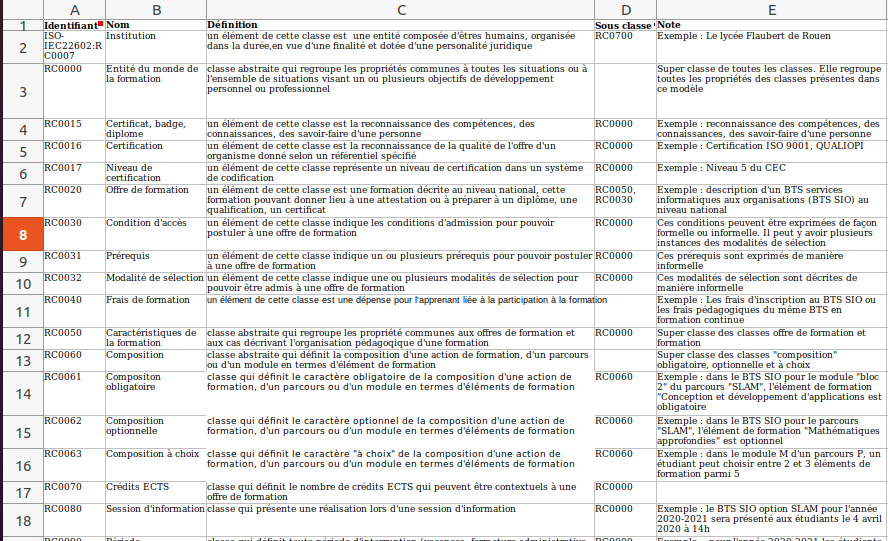
\includegraphics[width=13cm, height=6cm]{img/classes}
    \caption{Exemples de classes dans le fichier .ods modélisant le NoDEfr-2}
\end{figure}

Les propriétés sont définies dans les autres feuilles. Chaque feuille porte le nom de la classe dont les propriétés font réferences. Chaque ligne représente une propriété et chaque colonne un attribut de la propriété. Les attributs définis par le MLR pour les propriétés sont "Identifiant", "Nom", "Definition", "Indicateur linguistique", "Co domaine", "Régle de contenu", "Raffine", "Exemples, "Notes", "Cardinalité min", "Cardinalité max" et "Raison de l'ordonnancement".

\begin{figure}[!ht]
    \center
    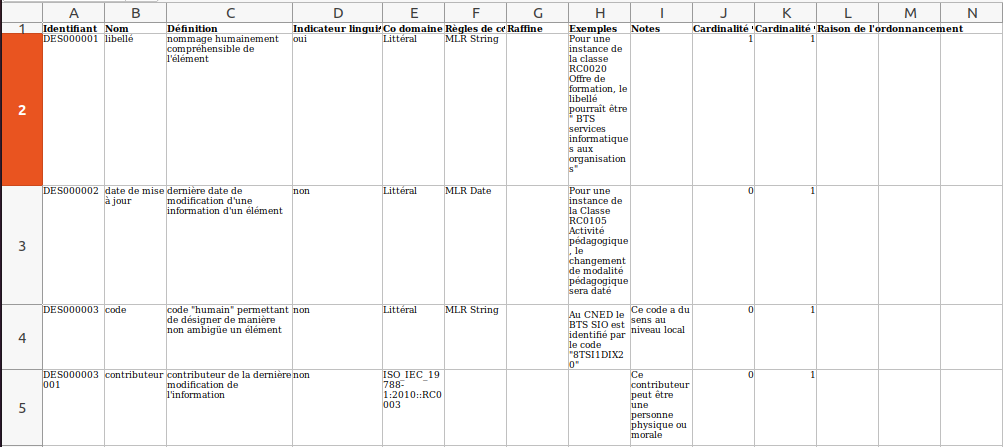
\includegraphics[width=13cm, height=6cm]{img/proprietes}
    \caption{Exemples de propriétés dans le fichier .ods modélisant le NoDEfr-2}
\end{figure}


La problématique du sujet est de formaliser automatiquement le travail réalisé par les experts de l'AFNOR en générant des schémas RDF et OWL. Pour cela, le sujet a été divisé en sous-sujet afin d'arriver à ces shémas "finaux". Tout d'abord la première étape était de développer une grammaire XSD pour valider des fichiers XML qui formaliseraient les classes et éléments de données du NoDEfr-2. La deuxième étape était donc de générer un fichier XML à partir du fichier .ods et qui respecte cette grammaire. Ensuite à partir de ce fichier XML il était possible de générer des schémas RDFS et OWL. 4 groupes distincts travaillaient donc sur le sujet, l'organisation était donc un point important.

\subsection{Le sujet de notre projet}

Le sous-sujet sur lequel nous avons travaillé est le 3ème, c'est à dire générer un shéma RDFS à partir du fichier XML.\\

Le RDF est un formalisme de représentation de métadonnées proposés le W3C. Il permet de décrire les ressources du Web, ce qui est utile notamment pour permettre le traitement automatique de ces données. Il est souvent représenté sous forme de triplet (sujet, prédicat, objet).

\begin{figure}[!ht]
    \center
    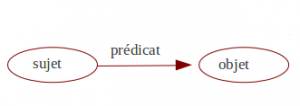
\includegraphics[width=8cm, height=3cm]{img/triplet}
    \caption{Triplet RDF}
\end{figure}

Le sujet est la ressource sur laquelle s'applique la métadonnée (donnée sur une donnée), le prédicat représente le nom de la métadonnée et l'objet est la valeur de la métadonnée. La collection de ces triplets permettent de former des schémas RDF. RDFS est lui une extension de RDF. Langage de description de RDF, il permet de fournir des élements de base afin de définir des ontologies et des vocabulaires RDF, en utilisant le système de classes et de propriétés.\\

\begin{figure}[!ht]
    \center
    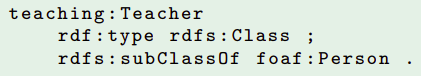
\includegraphics[width=6cm, height=2cm]{img/schema_rdfs}
    \caption{Définition d'une classe en RDFS}
\end{figure}

C'est à partir de ces informations (que nous avons vu dans les cours) que nous partions pour ce projet. Nous avions donc toutes les bases afin de réussir ce qui nous était demandé.

\section{Analyse et implémentation}

\subsection{Phase d'analyse et de recherche}
Dans la première phase du projet, nous avons réalisé beaucoup de recherches, tout d'abord pour nous familiariser avec les technologies utilisées (dont nous ne connaissions que les bases) et comprendre réellement ce qui était attendu. En effet, le sujet étant court il était important de bien comprendre ce qui était réellement demandé, notamment sur le type de schéma et la précision des informations demandées. Pour bien comprendre nous avons beaucoup utilisé les exemples disponibles sur internet et la documentation du W3C sur le RDF et le RDFS. Avec ces recherches nous avons identifié quelles propriétés RDF ou RDFS nous devions utiliser. Pour cela, la documentation W3C nous a été extrèmement utile. Pour chaque attribut des classes, nous avons regardé dans la documentation quelle pourrait être la propriété RDF et RDFS la plus adaptée. Même chose pour les propriétés.\\
\newcolumntype{M}[1]{>{\raggedright}m{#1}}
\begin{center}
    \begin{tabular}{| c | M{4cm} | M{3cm} | M{3cm} |}
        \hline
        Propriétés RDFS & Description W3C & Classes & Propriétés \tabularnewline
        \hline
        rdfs:type & used to state that a resource is an instance of a class. & rdfs:Class & rdf:Property  \tabularnewline
        \hline
        rdfs:label & used to provide a human-readable version of a resource's name & Nom de la classe & Nom de la propriété \tabularnewline
        \hline
        rdfs:comment & used to provide a human-readable description of a resource & Description de la classe & Description de la propriété  \tabularnewline
        \hline
        rdfs:subClassOf & used to state that all the instances of one class are instances of another & Sous-classes de la classe & X  \tabularnewline
        \hline
         rdfs:domain & used to state that any resource that has a given property is an instance of one or more classes & X & Classe à laquelle se réfère la propriété  \tabularnewline
        \hline
         rdfs:range & used to state that the values of a property are instances of one or more classes & X & Règle de contenu de la propriété  \tabularnewline
        \hline
     \end{tabular}
     Tableau présentant les propriétés RDFS que nous utilisons et leur correspondance dans le NoDEfr-2
 \end{center}

Nous avons également durant cette phase de recherche rédigé un petit fichier RDFS afin d'avoir un exemple de sortie que nous pourrions sortir.  Cela nous a permis de ne pas se lancer dans l'implémentation sans avoir une idée claire de ce que nous devions produire en sortie.\\

\begin{figure}[!ht]
    \center
    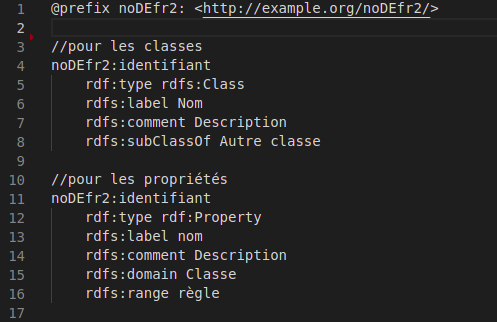
\includegraphics[width=9cm, height=5cm]{img/schema_ex}
    \caption{Fichier RDFS exemple}
\end{figure}

Nous nous sommes également familiarisé avec la syntaxe turtle car elle était imposée dans le sujet. Notre sortie devait donc être un fichier .ttl .\\

Nous avons également dû faire un choix concernant le langage de transformation XML que nous allions utiliser. En effet, notre sujet était de générer le schema RDFS à partir du fichier XML produit par l'équipe 2, il fallait donc trouver une technologie pour transformer le XML. Nous avons donc choisi d'utiliser le XSLT qui était la solution évidente au problème. Après des recherches sur d'autres langages de transformation XML, nous en avons conclu que XSLT était très utilisé, que nous l'avions déja vu en cours et que donc était la solution parfaite pour notre problématique.

\subsection{Implémentation}

Après nos recherches et le choix de nos technologies fait, nous avons dû implémenter notre solution.
Nous avons au départ identifié trois templates principaux (au sens XSLT) :
\begin{itemize} 
\item{un template à la racine pour mettre les préfixes au début de notre schéma}
\item{un template pour les classes}
\item{un template pour les relations}
\end{itemize}

Nous avons identifié 3 préfixes différents pour notre schéma. Ces préfixes devaient être placés au début du schéma donc le chemin XPATH pour ce template était simple puisque nous devions juste les mettre à la racine. Les deux premiers préfixes (rdf et rdfs) sont pour les propriétés rdf et rdfs, le troisième (nodefr2) est un préfixe pour notre modèle.

Afin de générer les classes de notre schéma, nous avons utilisé un template utilisant comme sélecteur "classe". Ainsi à chaque balise <classe> rencontrée dans le fichier XML nous allions pouvoir générer nos classes RDFS. Pour quelques propriétés (au sens RDF) nous avons utilisé d'autres templates spécialement pour les classes, essentiellement pour des raisons de propretés du code, en utilisant les "call-template". Nous avons géré dans ces templates l'affichage des valeurs des propriétés (avec les balises "xsl:value-of") mais également la vérification de l'existence des balises dans le XML(avec des balises "xsl:if"). En effet lors de nos premières versions du fichier XSLT il existait des propriétés vides (car par exemple il n'y a pas toujours de sous-classes) ce qui n'était pas possible pour avoir un schéma RDFS valide. Nous avons dû également gérer le cas où il y a plusieurs sous-classes, en utilisant les expressions XPath "substring-before" et "substring-after".

\begin{figure}[!ht]
    \center
    \centerline{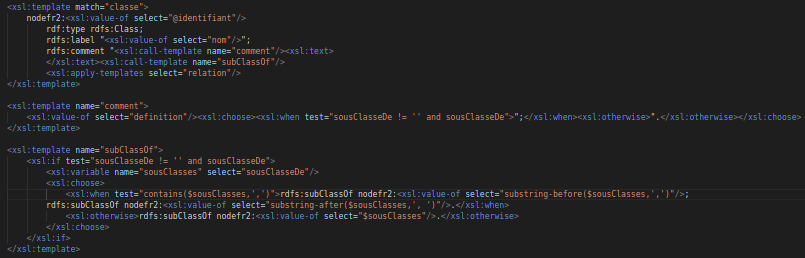
\includegraphics[scale=0.5,width=18cm, height=6cm]{img/temp_classes}}
    \caption{Templates pour les classes dans le XSLT}
\end{figure}

Nous avons utilisé les mêmes techniques pour les propriétés de notre schéma (ce qui correspond aux relations dans le fichier XML).

\begin{figure}[!ht]
    \center
    \centerline{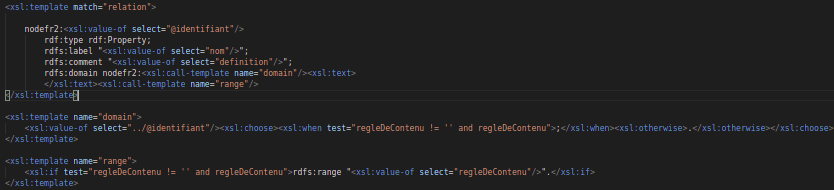
\includegraphics[scale=0.5,width=19cm, height=6cm]{img/temp_proprietes}}
    \caption{Templates pour les propriétés dans le XSLT}
\end{figure}

\subsection{Difficultés rencontrées}

Nous avons rencontré deux principales difficultés lors de l'implémentation. La première était les points virgules et les points qui se situent en fin des lignes. En effet, le point doit être mis seulement sur la dernière ligne, or la dernière ligne de la définition des classes et des propriétés ne sont pas toujours pour la même propriété : par exemple une classe ne se termine pas forcément par la définition de la sous-classe (car certaines classes n'ont pas de sous-classes) donc dans ce cas le point doit se situer à la fin de la ligne qui définit "rdfs:comment". Pour régler ce problème nous avons utilisé des balises "xsl:choose" qui permet de faire une structure conditionnelle. Dans le cas où l'élément "sousClasseDe" existait pour cette classe, alors on place un point-virgule sur la ligne de définition de la propriété "rdfs:comment", sinon on met un point. Nous avons eu le même problème avec l'élément "regleDeContenu" pour les propriétés que nous avons réglé de la même façon. Une autre solution consistait simplement à ne pas mettre les éléments non obligatoires à la fin des définitions des classes ou des propriétés, mais nous avions déja implémenté l'autre solution quand nous nous en sommes rendu compte et nous avons préféré garder celle-ci afin d'être raccord avec le schéma de sortie que nous avions réalisé précédemment. \\

La deuxième difficulté rencontrée est sur les éléments "sousClasseDe". En effet la valeur de la propriété "rdfs:subClassOf" devait être "nodefr2:idclasse", or il peut y avoir plusieurs sous-classes et donc plusieurs "rdfs:subClassOf" dans la définition d'une classe. Le problème était que dans le XML les sous-classes étaient toutes dans un même élement <sousClasseDe> séparées par des virgules. Nous avons donc dû rechercher un moyen de faire un traitement de chaines de caractères, afin de séparer les id des classes entre les virgules. Nous avons utilisé pour cela les fonction XPath "substring-before" et "substring-after", qui permettent d'avoir la sous-chaîne avant et après un certain caractère (dans notre cas la virgule). Les éléments "sousClasseDe" contenant au maximum 2 sous-classes, ces deux fonctions étaient suffisantes pour régler notre problème (avec l'utilisation de "xsl:choose" et des variables).\\

D'autres petites difficultés ont également émergé, comme par exemple pour la mise en page. Nous voulions une mise en page de fichier .ttl qui soit cohérente et bien indenté. Malheureusement ce n'est pas parfait, notamment en raison de certains "rdfs:comment" dans la définition des classes, où le point et les guillements sont mis une ligne en dessous. Cela est causé par le fichier XML, lorsque la balise </description> n'est pas directement collée à la fin de la phrase mais mis une ligne en dessous.

\subsection{Collaboration avec les autres groupes}

La collaboration avec les autres groupe étaient très importantes lors de notre travail. En effet, la sortie du travail d'un  groupe est l'entrée du travail du groupe suivant. 

\begin{figure}[!ht]
    \center
    \centerline{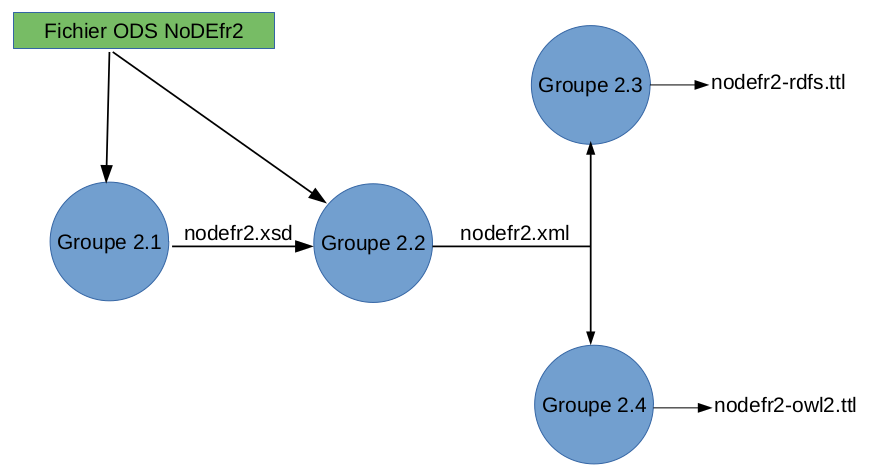
\includegraphics[width=12cm,height=6cm]{img/schema_groupes}}
    \caption{Schéma modélisant les entrées/sorties des groupes}
\end{figure}

Nous devions donc nous organiser afin que les derniers groupes ne commencent pas leur projet une fois le travail des groupes précédents terminé. Pour cela, le premier groupe a créé un serveur Discord afin que nous puissions communiquer. Nous avons organisé régulièrement des petites réunions avec tous les groupes ou seulement certains, pour mettre au clair certains points et se coordonner.

Dans notre cas, nous avions surtout besoin de la sortie du groupe qui produisait le fichier XML. Il a donc fallu bien se mettre d'accord sur la sortie qu'ils allaient produire afin que nous puissions avancer de notre côté, en créant un fichier XML exemple reprennant ce qu'ils allaient produire mais seulement avec une partie des données (cf annexe 1).

Nous avons également beaucoup parlé avec le groupe produisant le shéma OWL, vu qu'ils travaillaient au même niveau que nous. Nous avons pu discuter de ce que nous devions produire et des différences entre nos deux schémas. 

\newpage
\section{Conclusion}
Ce projet aura été formateur, tant sur le plan technique que relationnel. Nous avons pu mettre en pratique sur un vrai cas concret les connaissances que nous avons apprises sur le web sémantique et le web des données. Les technologies utilisées sont très intéréssantes et ce projet aura justement permis de mieux comprendre dans quel cadre elles sont utilisées. Le fonctionnement en sujet/sous-sujet nous aura permis de plus s'organiser en amont et nous pousse à ne pas commencer le projet trop tard, même si c'est parfois un peu difficile pour les groupes étant au bout de la chaine (qui sont obligés de travailler sur des "faux" exemples amenés à être modifié).

Concernant notre travail nous sommes plutôt satisfait de ce que nous avons réalisé. Nous pensons que le schéma RDFS généré avec le fichier XML est correcte et représente correctement les informations du NoDEfr-2.

\newpage
\section{Annexes}
\subsection{Annexe 1 : première version du fichier XML exemple}

\begin{figure}[!ht]
    \centering
    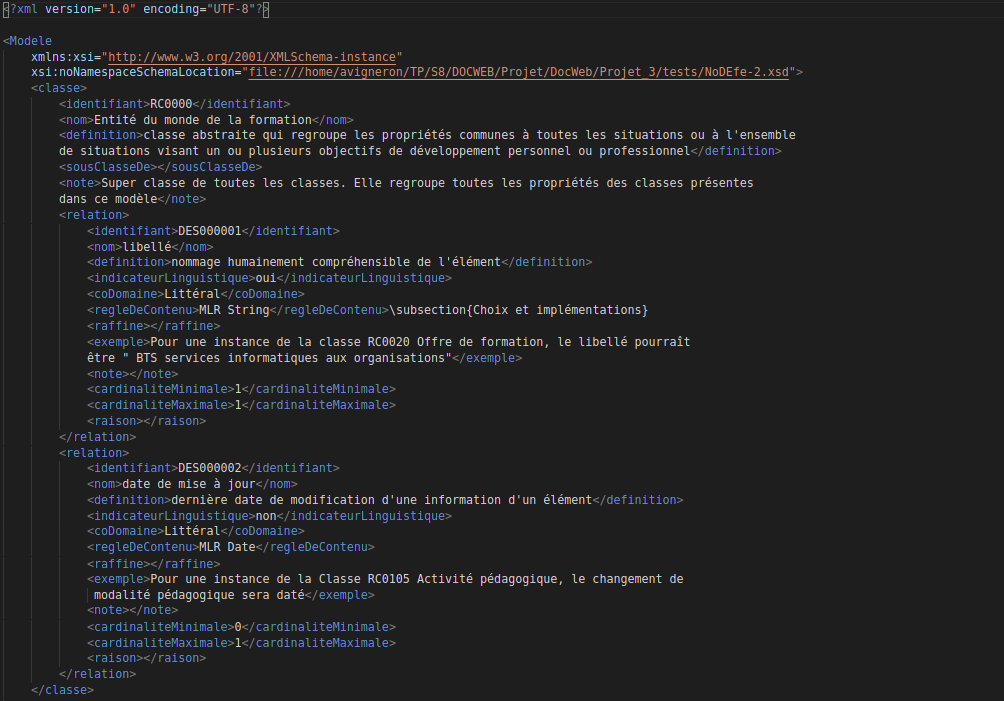
\includegraphics[scale=0.5,width=18cm, height=16cm]{img/ex_xml_1}
\end{figure}

\newpage
\begin{figure}[!ht]
    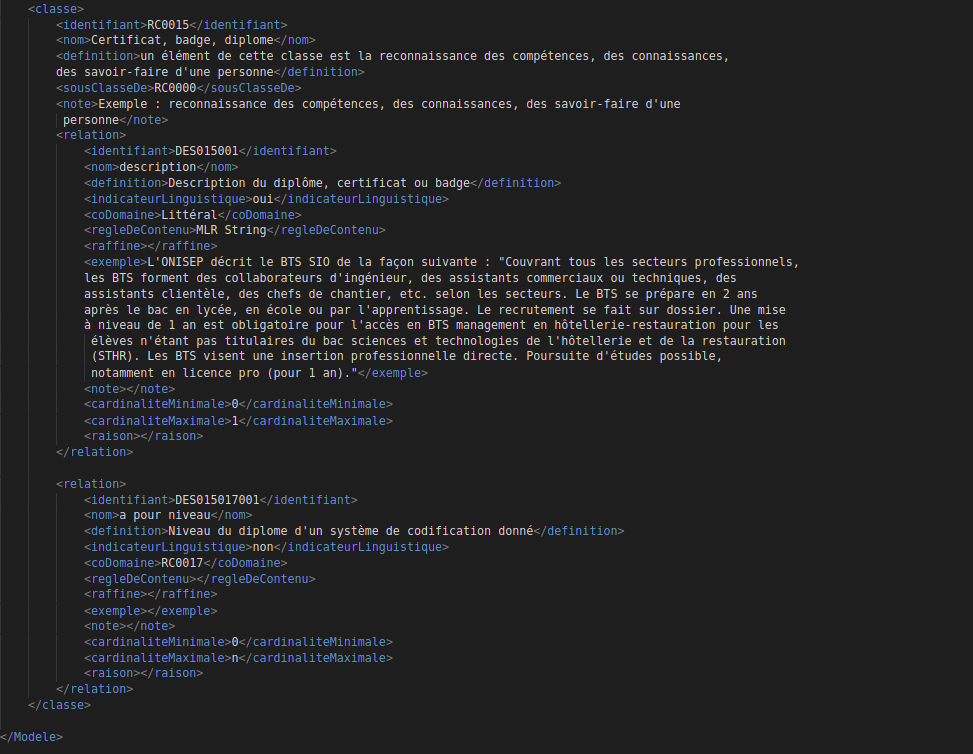
\includegraphics[scale=0.5,width=18cm, height=16cm]{img/ex_xml_2}
\end{figure}

\newpage
\subsection{Annexe 2 : fichier XSLT}
\begin{figure}[!ht]
    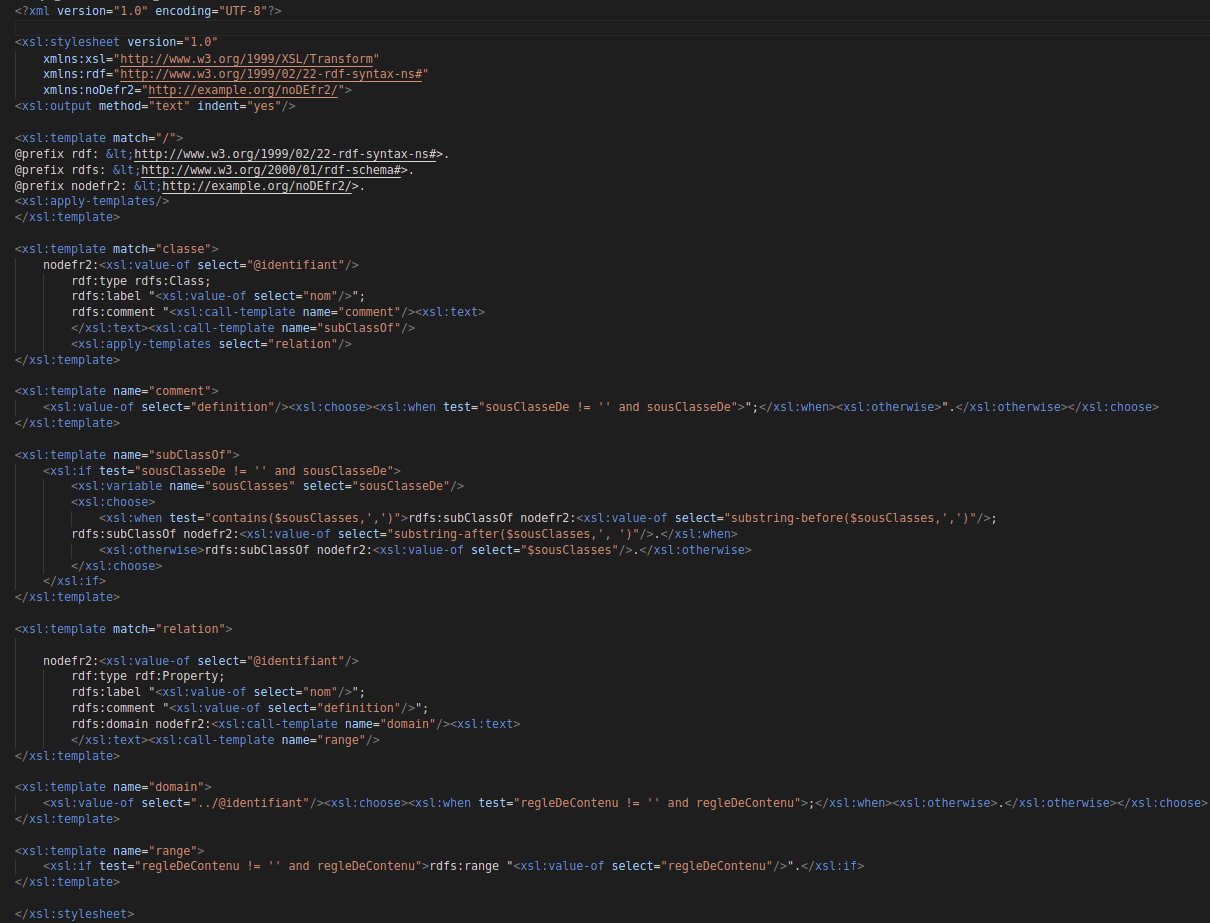
\includegraphics[scale=0.5,width=16cm, height=13cm]{img/xslt}
\end{figure}

\newpage
\section{Webographie}
\normalsize
Yolaine Bourda, Gilles Gauthier, Rosa-Maria Gomez de Regil, Olivier Catteau. \textbf{Métadonnées pour
ressources d’apprentissage (MLR) : nouvelle norme ISO de description de ressources pédagogiques.}
STICEF (Sciences et Technologies de l’Information et de la Communication pour l’Éducation et la
Formation), ATIEF, 2010, 17, 11 p. ffhal-00696450f\\
\\
$[www.w3.org]$ \textbf{"RDF Schema 1.1"}
, https://www.w3.org/TR/rdf-schema/\\
\\
$[www.w3.org]$ \textbf{"RDF Primer"}
, https://www.w3.org/TR/rdf-primer/\\
\\
$[moodle.insa-rouen.fr]$ Nicolas Delestre, Nicolas Malandain \textbf{"XSLT"}
, https://moodle.insa-rouen.fr/pluginfile.php/133451/mod\_resource/content/1/XSLT.pdf\\
\\
$[moodle.insa-rouen.fr]$ Nicolas Delestre, Nicolas Malandain \textbf{"RDF-SPARQL"}
, https://moodle.insa-rouen.fr/pluginfile.php/133458/mod\_resource/content/1/RDF-SPARQL.pdf\\
\\
$[moodle.insa-rouen.fr]$ Nicolas Delestre, Nicolas Malandain \textbf{"RDFS-OWL"}
, https://moodle.insa-rouen.fr/pluginfile.php/133459/mod\_resource/content/2/RDFS-OWL.pdf\\
\\
$[blog.onyme.com,2011]$ Marina Soler, \textbf{"Les ontologies informatiques : l'exemple par OWL et autres"}
, http://blog.onyme.com/les-ontologies-informatiques-lexemple-par-owl-et-autres/\\
\\
$[www.w3.org]$ \textbf{"RDF Schema 1.1"}
, https://www.w3.org/TR/rdf-schema/\\
\\
$[lms.fun-mooc.fr]$Inria, \textbf{"le modèle de données RDF"}
, https://lms.fun-mooc.fr/c4x/inria/41002S02/asset/C013FG-W2.pdf\\
\\
$[edutechwiki.unige.ch]$, \textbf{"Tutoriel XSLT débutant"}
, http://edutechwiki.unige.ch/fr/Tutoriel\_XSLT\\
\\
$[perso.univ-mlv.fr]$ O.Curé,\textbf{"RDF"}
, http://perso.univ-mlv.fr/ocure/RDF.pdf\\
\\
$[www.fil.univ-lille1.fr]$ Anne-Cécile Caron,\textbf{"Vocabulaire RDF : RDFS"}
, https://www.fil.univ-lille1.fr/~caronc/WS/rdfsPar4.pdf\\
\\
$[www.info.univ-angers.fr]$ \textbf{"RDF-Schema"}
, http://www.info.univ-angers.fr/pub/genest/fichiers/
m1\_websem/ws\_chap4.pdf\\
\end{document}
